\section{1174066 - D.Irga B. Naufal Fakhri}
\subsection{Teori}
\subsubsection{Jelaskan kenapa kata-kata harus di lakukan vektorisasi}

\hfill\break
Kata kata harus dilakukan vektorisasi dikarenakan atau bertujuan utk mengukur nilai kemunculan suatau kata yang serupa dari sebuah kalimat sehingga kata-kata tersebut dapat di prediksi kemunculanya. atau juga di buatnya vektorisasi data digunakan untuk memprediksi bobot dari suatu kata misalkan ayam dan kucing sama-sama hewan maka akan dibuat prediksi apakah kata tersebut akan muncul pada kalimat yang kira-kira memiliki bobot yang sama.
\begin{figure}[H]
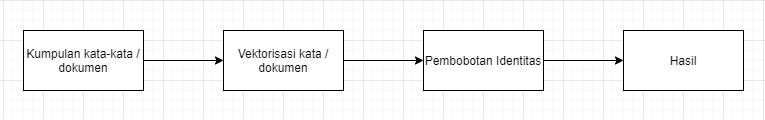
\includegraphics[width=4cm]{figures/1174066/5/1.jpg}
\centering
\caption{Teori 1}
\end{figure}

\subsubsection{Jelaskan mengapa dimensi dari vektor dataset google bisa sampai 300.}

\hfill\break
Karena setiap objek memiliki identitas khusus, misalnya sederhana. Dalam dataset Google ini memiliki 3 objek, kucing, anjing, dan ember yang disetujui. Kemudian dari masing-masing objek dibandingkan dataset antara kucing dan anjing kemudian kucing dan ember. Hasil yang diperoleh untuk kucing dan anjing sekitar 75\% sedangkan untuk kucing dan ember yang memiliki persentase 15\%. Untuk lebih lengkapnya bisa dilihat pada gambar berikut: 
\begin{figure}[H]
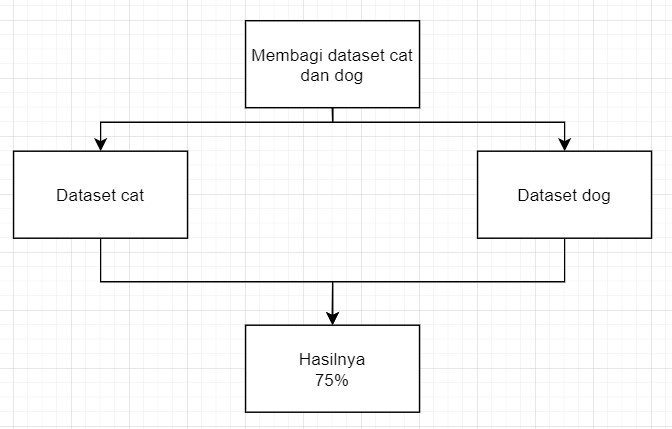
\includegraphics[width=4cm]{figures/1174066/5/2.jpg}
\centering
\caption{Teori 2}
\end{figure}

\subsubsection{Jelaskan konsep vektorisasi untuk kata}

\hfill\break
Konsep untuk vektorisasi kata sama dengan masukan atau input pada kata-kata di mesin pencari. Maka anggaplah itu akan dikeluarkan sebagai saran tentang kata tersebut. Jadi kata data diperoleh dari hasil yang diolah dalam kalimat sebelumnya yang telah diproses. Contoh sederhana dalam kalimat berikut (Please Subscribe and Turn on Notification Bell), dalam kalimat itu terkait dengan kalimat saluran, kata akan dibuat data pelatihan untuk mesin. Jadi kita kompilasi kata channel, maka mesin akan menampilkan hubungannya dengan kata tersebut. Contoh ilustrasi sederhananya seperti berikut:
\begin{figure}[H]
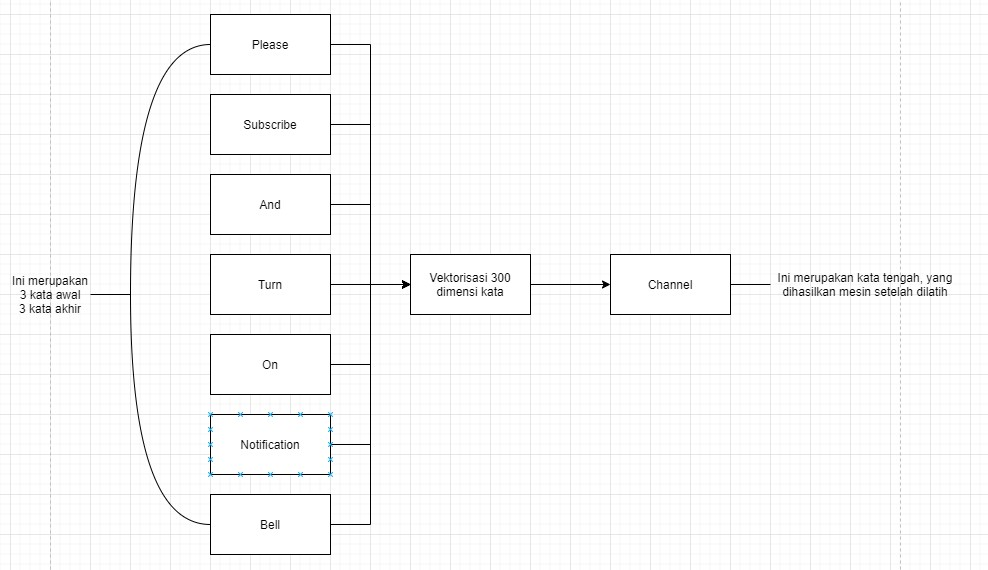
\includegraphics[width=4cm]{figures/1174066/5/3.jpg}
\centering
\caption{Teori 3}
\end{figure}

\subsubsection{Jelaskan konsep vektorisasi untuk dokumen}	
\hfill\break
Sama halnya dengan vektorisasi kata, yang membedakan hanya pada proses awalnya. Untuk vektorisasi dokumen ini, mesin akan membaca semua kalimat yang terdapat pada dokumen tersebut, lalu kalimat yang terdapat pada dokumen akan di pecah menjadi kata-kata. Perhatikan gambar berikut: 
\begin{figure}[H]
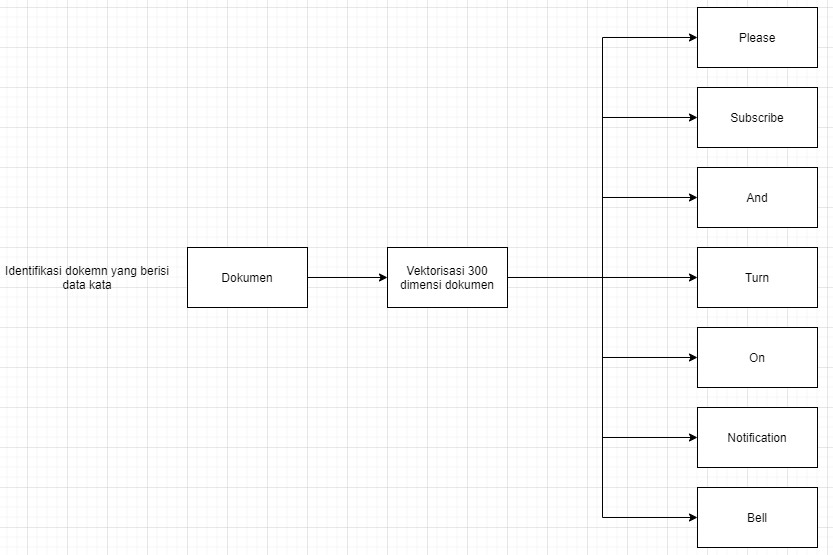
\includegraphics[width=4cm]{figures/1174066/5/4.jpg}
\centering
\caption{Teori 4}
\end{figure}

\subsubsection{Jelaskan apa mean dan standar deviasi}
\hfill\break
Mean adalah nilai rata-rata. Untuk mendapatkan makna ini, kita hanya perlu menambahkan data yang tersedia dan kemudian membaginya dengan jumlah data. Sedangkan standar deviasi adalah nilai statistik yang digunakan untuk menentukan bagaimana data didistribusikan dalam sampel, dan menentukan titik data individu dengan nilai rata-rata nilai sampel. Rumusnya ialah sebagai berikut:
\begin{figure}[H]
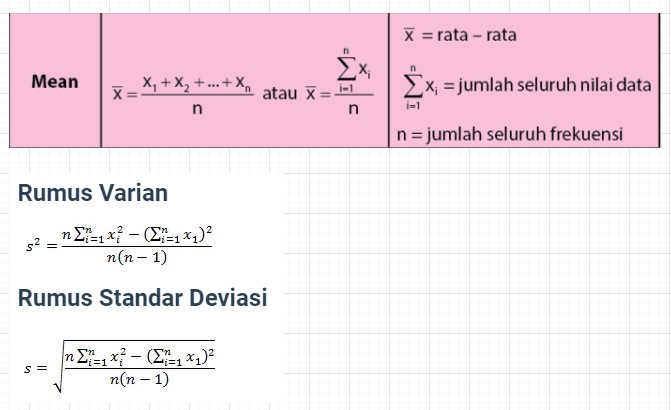
\includegraphics[width=4cm]{figures/1174066/5/5.jpg}
\centering
\caption{Teori 5}
\end{figure}

\subsubsection{Jelaskan apa itu skip-gram}
\hfill\break
Skip-gram sama halnya dengan vektorisasi kata, namun untuk skip-gram ia dibalik prosesnya. Yang sebelumnya dari kalimat lalu di olah untuk menemukan salah satu kata, kali ini dari keyword tersebut akan diolah menjadi suatu kalimat yang memiliki keterkaitannya dengan keyword tersebut. Contoh sederhananya seperti gambar berikut: 
\begin{figure}[H]
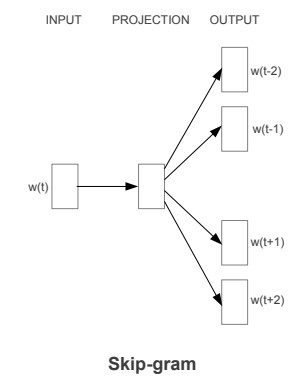
\includegraphics[width=4cm]{figures/1174066/5/6.jpg}
\centering
\caption{Teori 6}
\end{figure}

\subsection{Praktek}
\subsubsection{Nomor 1}

\hfill\break
\lstinputlisting[firstline=8, lastline=10]{src/1174066/5/1.py}
Kode digunakan untuk import library gensim. Gensim itu sendiri berguna untuk melakukan pemodelan dengan dataset atau topik yang telah ditentukan. Untuk keluaran 100 logging itu library opsional karena logging hanya untuk menampilkan berupa log untuk setiap code yang dijalankan. Dan keluaran 101 itu hasil load data dari file vektor google itu, disini saya menggunakan limit karena kondisi laptop yang tidak mempuni untuk melakukan running data sebesar 3 juta file, jadi saya batasi hanya melakukan running 500 ribu data saja, hasilnya ialah sebagai berikut: 
\begin{figure}[H]
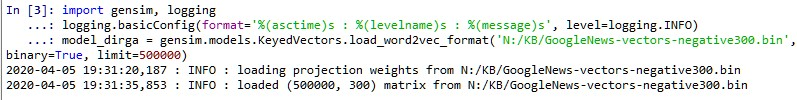
\includegraphics[width=4cm]{figures/1174066/5/hasil1-1.jpg}
\centering
\caption{Hasil dari Nomor 1-1}
\end{figure}

\hfill\break
\lstinputlisting[firstline=13, lastline=33]{src/1174066/5/1.py}
Menampilkan data hasil vektorisasi data:
\begin{figure}[H]
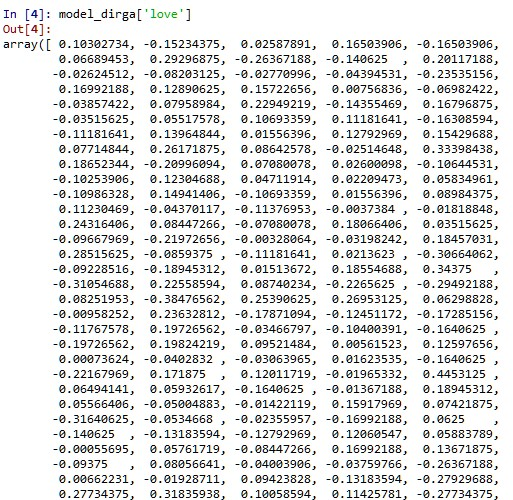
\includegraphics[width=4cm]{figures/1174066/5/hasil1-2.jpg}
\centering
\caption{Data love}
\end{figure}

\hfill\break
\begin{figure}[H]
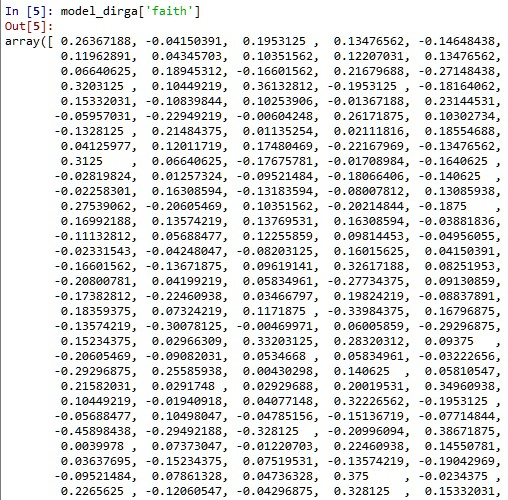
\includegraphics[width=4cm]{figures/1174066/5/hasil1-3.jpg}
\centering
\caption{Data faith}
\end{figure}

\hfill\break
\begin{figure}[H]
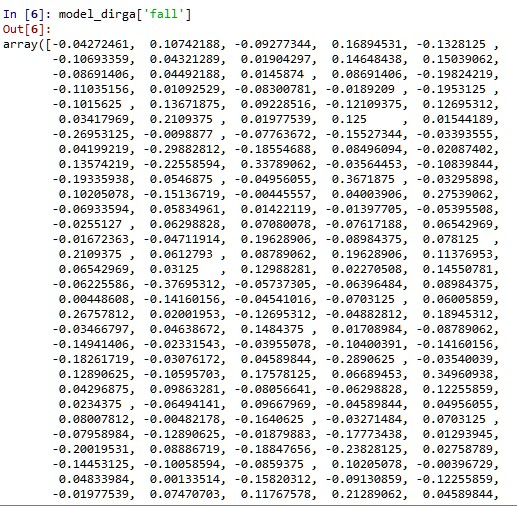
\includegraphics[width=4cm]{figures/1174066/5/hasil1-4.jpg}
\centering
\caption{Data fall}
\end{figure}

\hfill\break
\begin{figure}[H]
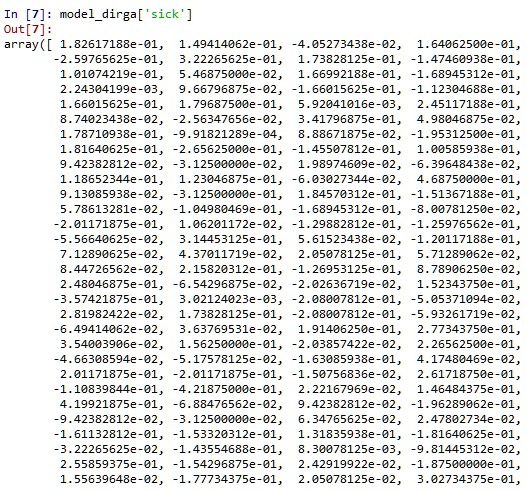
\includegraphics[width=4cm]{figures/1174066/5/hasil1-5.jpg}
\centering
\caption{Data sick}
\end{figure}

\hfill\break
\begin{figure}[H]
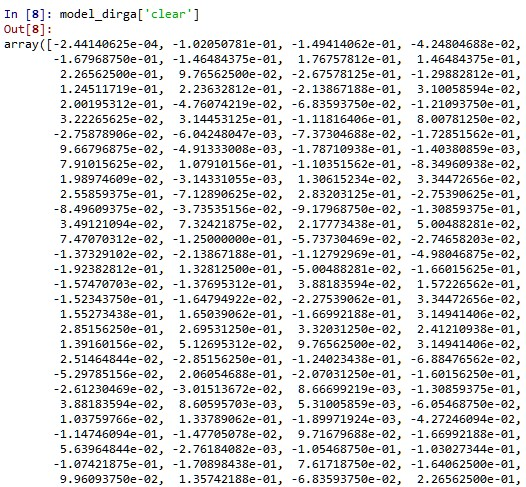
\includegraphics[width=4cm]{figures/1174066/5/hasil1-6.jpg}
\centering
\caption{Data clear}
\end{figure}

\hfill\break
\begin{figure}[H]
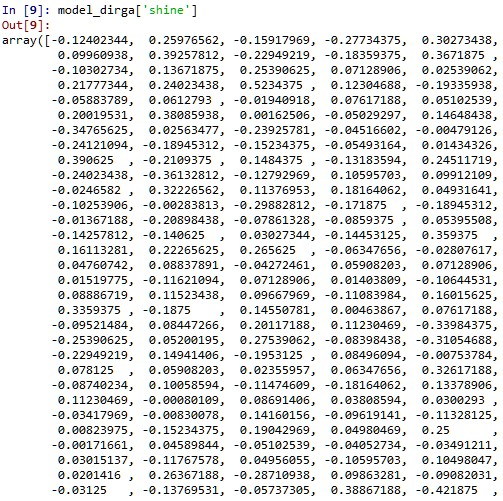
\includegraphics[width=4cm]{figures/1174066/5/hasil1-7.jpg}
\centering
\caption{Data shine}
\end{figure}

\hfill\break
\begin{figure}[H]
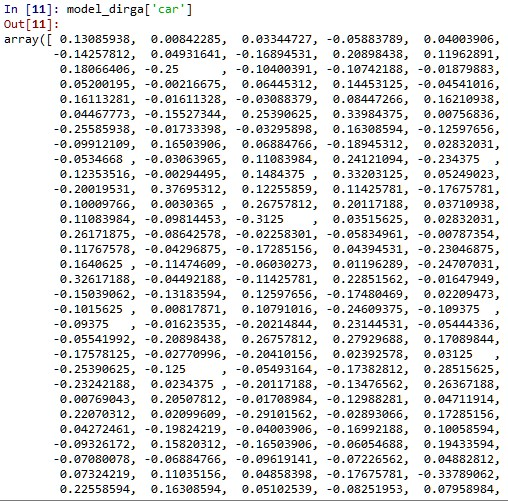
\includegraphics[width=4cm]{figures/1174066/5/hasil1-8.jpg}
\centering
\caption{Data bag}
\end{figure}

\hfill\break
\begin{figure}[H]
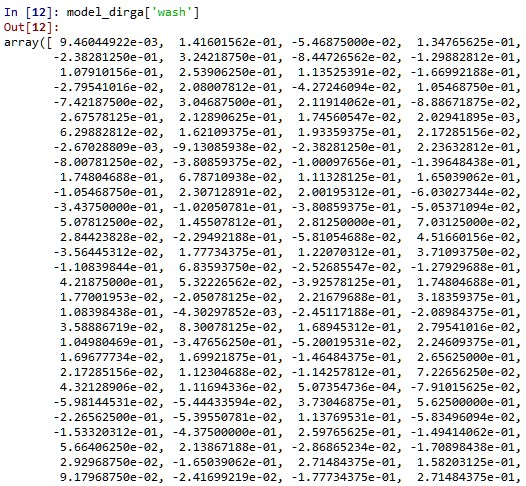
\includegraphics[width=4cm]{figures/1174066/5/hasil1-9.jpg}
\centering
\caption{Data car}
\end{figure}

\hfill\break
\begin{figure}[H]
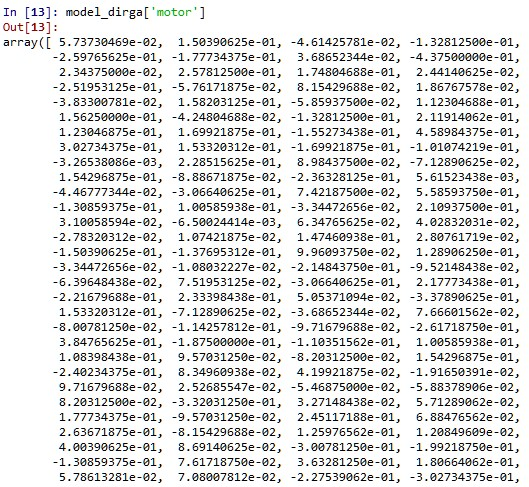
\includegraphics[width=4cm]{figures/1174066/5/hasil1-10.jpg}
\centering
\caption{Data wash}
\end{figure}

\hfill\break
\begin{figure}[H]
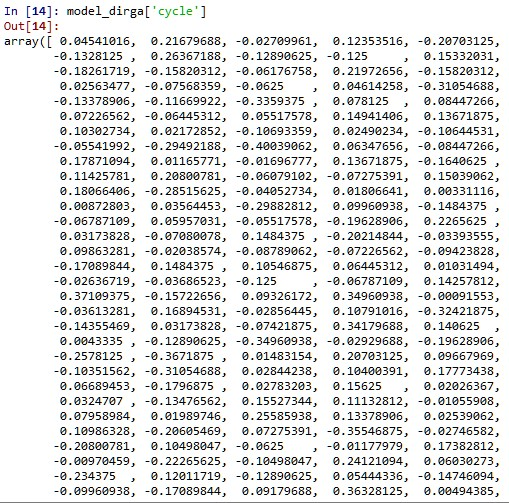
\includegraphics[width=4cm]{figures/1174066/5/hasil1-11.jpg}
\centering
\caption{Data motor}
\end{figure}

\hfill\break
\begin{figure}[H]
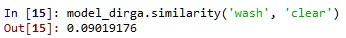
\includegraphics[width=4cm]{figures/1174066/5/hasil1-12.jpg}
\centering
\caption{Data cycle}
\end{figure}

\lstinputlisting[firstline=35, lastline=43]{src/1174066/5/1.py}
Merupakan persentase dari perbandingan kata:
\hfill\break
\begin{figure}[H]
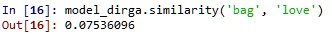
\includegraphics[width=4cm]{figures/1174066/5/hasil1-13.jpg}
\centering
\caption{Data wash dan clear}
\end{figure}

\hfill\break
\begin{figure}[H]
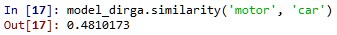
\includegraphics[width=4cm]{figures/1174066/5/hasil1-14.jpg}
\centering
\caption{Data bag dan love}
\end{figure}

\hfill\break
\begin{figure}[H]
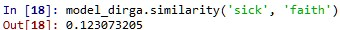
\includegraphics[width=4cm]{figures/1174066/5/hasil1-15.jpg}
\centering
\caption{Data sick dan faith}
\end{figure}

\hfill\break
\begin{figure}[H]
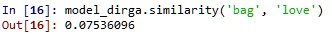
\includegraphics[width=4cm]{figures/1174066/5/hasil1-13.jpg}
\centering
\caption{Data cycle dan shine}
\end{figure}


\subsubsection{Nomor 2}
\hfill\break
\lstinputlisting[firstline=46, lastline=52]{src/1174066/5/1.py}
Kode ini berguna untuk membuat string memakai import re, dengan memakai test\_string sebagai datanya
\begin{figure}[H]
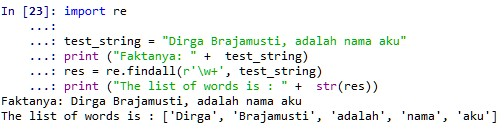
\includegraphics[width=4cm]{figures/1174066/5/hasil2.jpg}
\centering
\caption{Nomor 2}
\end{figure}
\lstinputlisting[firstline=53, lastline=58]{src/1174066/5/1.py}
Kode ini berguna untuk membuat string dengan import random, memakai variable sent\_matrix untuk membuat string, dan result sebagai print dari random data yang diacak, hasilnya akan berubah-ubah:
\begin{figure}[H]
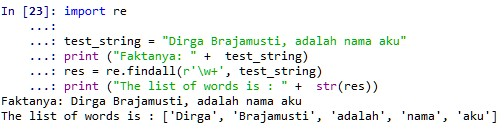
\includegraphics[width=4cm]{figures/1174066/5/hasil2.jpg}
\centering
\caption{Nomor 2-1}
\end{figure}

\subsubsection{Nomor 3}
\hfill\break
\lstinputlisting[firstline=60, lastline=70]{src/1174066/5/1.py}
Fungsi dari library gensim untuk pemodelan topik unsupervised learning. Fungsi dari doc2vec itu sendiri adalah untuk membandingkan bobot data yang terdapat pada dokumen lainnya, apakah kata-katanya ada yang sama atau tidak. Lalu untuk tagged document itu memasukan kata-kata pada setiap dokumennya untuk di vektorisasi, dan model untuk membuat model dan save file model.
\begin{figure}[H]
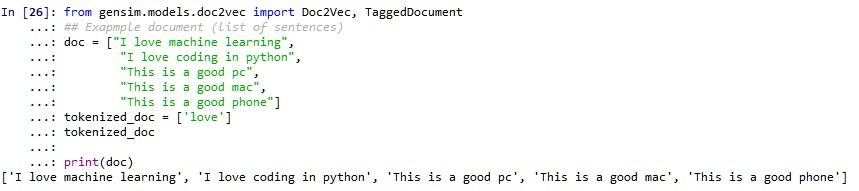
\includegraphics[width=4cm]{figures/1174066/5/hasil3.jpg}
\centering
\caption{Nomor 3}
\end{figure}
\lstinputlisting[firstline=73, lastline=82]{src/1174066/5/1.py}
\begin{figure}[H]
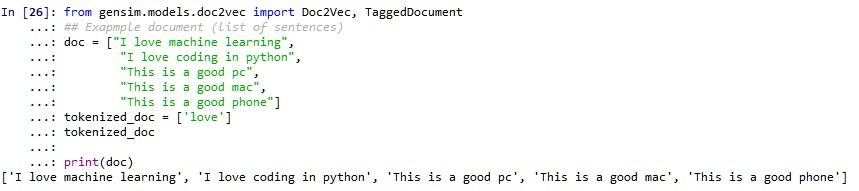
\includegraphics[width=4cm]{figures/1174066/5/hasil3.jpg}
\centering
\caption{Nomor 3-1}
\end{figure}	

\subsubsection{Nomor 4}
\hfill\break
\lstinputlisting[firstline=86, lastline=97]{src/1174066/5/1.py}
Disini memakai dataset dari aclImdb. Untuk menambahkan data training kita melakukan import library os, library os fungsinya untuk melakukan interaksi antara python dengan windows atau os kita, setelah itu buat variable unsup sentences. Lalu pilih direktori tempat data akan disimpan. Lalu untuk mensortir data yang terdapat pada folder aclImdb dan membaca file tersebut dengan ektensi .txt. Hasil dari code pertama tersebut adalah adanya data hasil running dari folder aclImdb.
\begin{figure}[H]
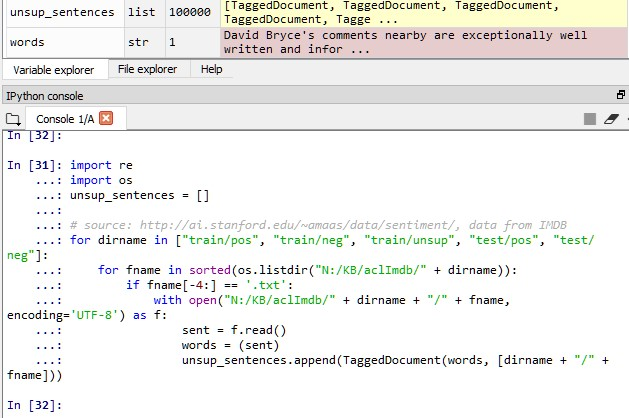
\includegraphics[width=4cm]{figures/1174066/5/hasil4.jpg}
\centering
\caption{Nomor 4}
\end{figure}		

\subsubsection{Nomor 5}
\hfill\break
\lstinputlisting[firstline=101, lastline=105]{src/1174066/5/1.py}
Pada bagian pengacakan data berguna untuk mengacak data agar saat data di running bisa berjalan lebih baik dan hasil presentase akan lebih baik. Sedangkan untuk pembersihan data untuk memberikan ruang bagi ram laptop kita setelah melakukan running data lebih dari 3 juta , agar lebih ringan saat proses selanjutnya.
\begin{figure}[H]
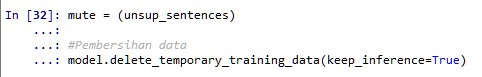
\includegraphics[width=4cm]{figures/1174066/5/hasil5.jpg}
\centering
\caption{Nomor 5}
\end{figure}	

\subsubsection{Nomor 6}
\hfill\break
\lstinputlisting[firstline=109, lastline=113]{src/1174066/5/1.py}
Save berfungsi untuk menyimpan hasil dari proses pelatihan data sebelumnya ke dalam sebuah file, model tersebut dilakukan penyimpanan untuk memberikan keringanan pada ram agar saat akan melakukan pelatihan lagi, model tersebut bisa load tanpa harus melakukan pelatihan dari awal dan akan menghemat waktu. Sedangkan untuk delete temporary training data ini berfungsi untuk menghapus data latihan yang sebelumnya sudah dilakukan dan disimpan, bertujuan untuk memberikan keringanan pada ram. Karena setelah melakukan proses pelatihan ram biasanya jadi penuh sampai komputer menjadi lag. Itulah fungsi dari delete temporary training data
\begin{figure}[H]
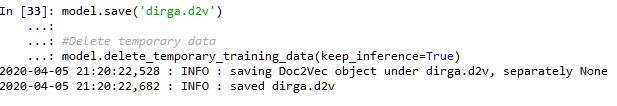
\includegraphics[width=4cm]{figures/1174066/5/hasil6.jpg}
\centering
\caption{Nomor 6}
\end{figure}

\subsubsection{Nomor 7}
\hfill\break
\lstinputlisting[firstline=116, lastline=116]{src/1174066/5/1.py}
Infer\_vector berfungsi untuk membandingkan kata yang tercantum dengan vektor yang mana pada dokumen yang sudah diload pada step sebelumnya. Selain itu infer\_vector juga untuk menghitung atau mengkalkulasikan vektor dari kata yang dicantumkan dari model yang telah dibuat. Alangkah baiknya kata yang dicantumkan itu lebih panjang lagi agar hasilnya bisa lebih baik lagi. 
\begin{figure}[H]
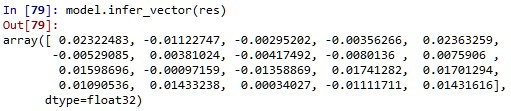
\includegraphics[width=4cm]{figures/1174066/5/hasil7.jpg}
\centering
\caption{Nomor 7}
\end{figure}

\subsubsection{Nomor 8}
\hfill\break
\lstinputlisting[firstline=119, lastline=122]{src/1174066/5/1.py}
Cosine\_similarity berfungsi untuk membandingkan vektorisasi data diantara kedua kata yang di inputkan, jika hasil presentase dari kedua kata tersebut lebih dari 50\% itu memiliki kemungkinan kata tersebut terdapat dalam 1 file. Namun jika kurang dari 50\% itu kemungkinan kata tersebut tidak terdapat dalam 1 file. Hasil yang didapatkan pada code tersebut hanya 0.49\% itu dikarenakan kata pertama dan kedua tidak memiliki kesamaan vektorisasi dan tidak terdapat pada salah satu dokumen.
\begin{figure}[H]
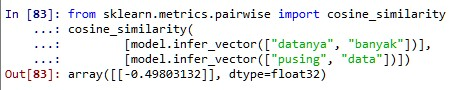
\includegraphics[width=4cm]{figures/1174066/5/hasil8.jpg}
\centering
\caption{Nomor 8}
\end{figure}

	
\subsubsection{Nomor 9}
\hfill\break
\lstinputlisting[firstline=125, lastline=131]{src/1174066/5/1.py}
Melakukan perhitungan presentase dengan menggunakan cross\_validation dengan metode kneighborsClassifier. Menggunakan dataset iris
\begin{figure}[H]
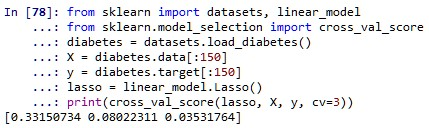
\includegraphics[width=4cm]{figures/1174066/5/hasil9.jpg}
\centering
\caption{Nomor 9}
\end{figure}


\subsection{Penanganan Error}
\begin{itemize}
\item Error
\begin{enumerate}
\item FileNotFoundError
\begin{figure}[H]
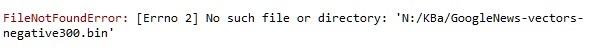
\includegraphics[width=4cm]{figures/1174066/5/error1.jpg}
\centering
\caption{Error 1}
\end{figure}
\end{enumerate}
\item Solusi
\begin{enumerate}
\item FileNotFoundError

Perhatikan letak file ada dimana, pastikan path telah benar
\end{enumerate}
\end{itemize}

\subsection{Bukti Tidak Plagiat}
\begin{figure}[H]
	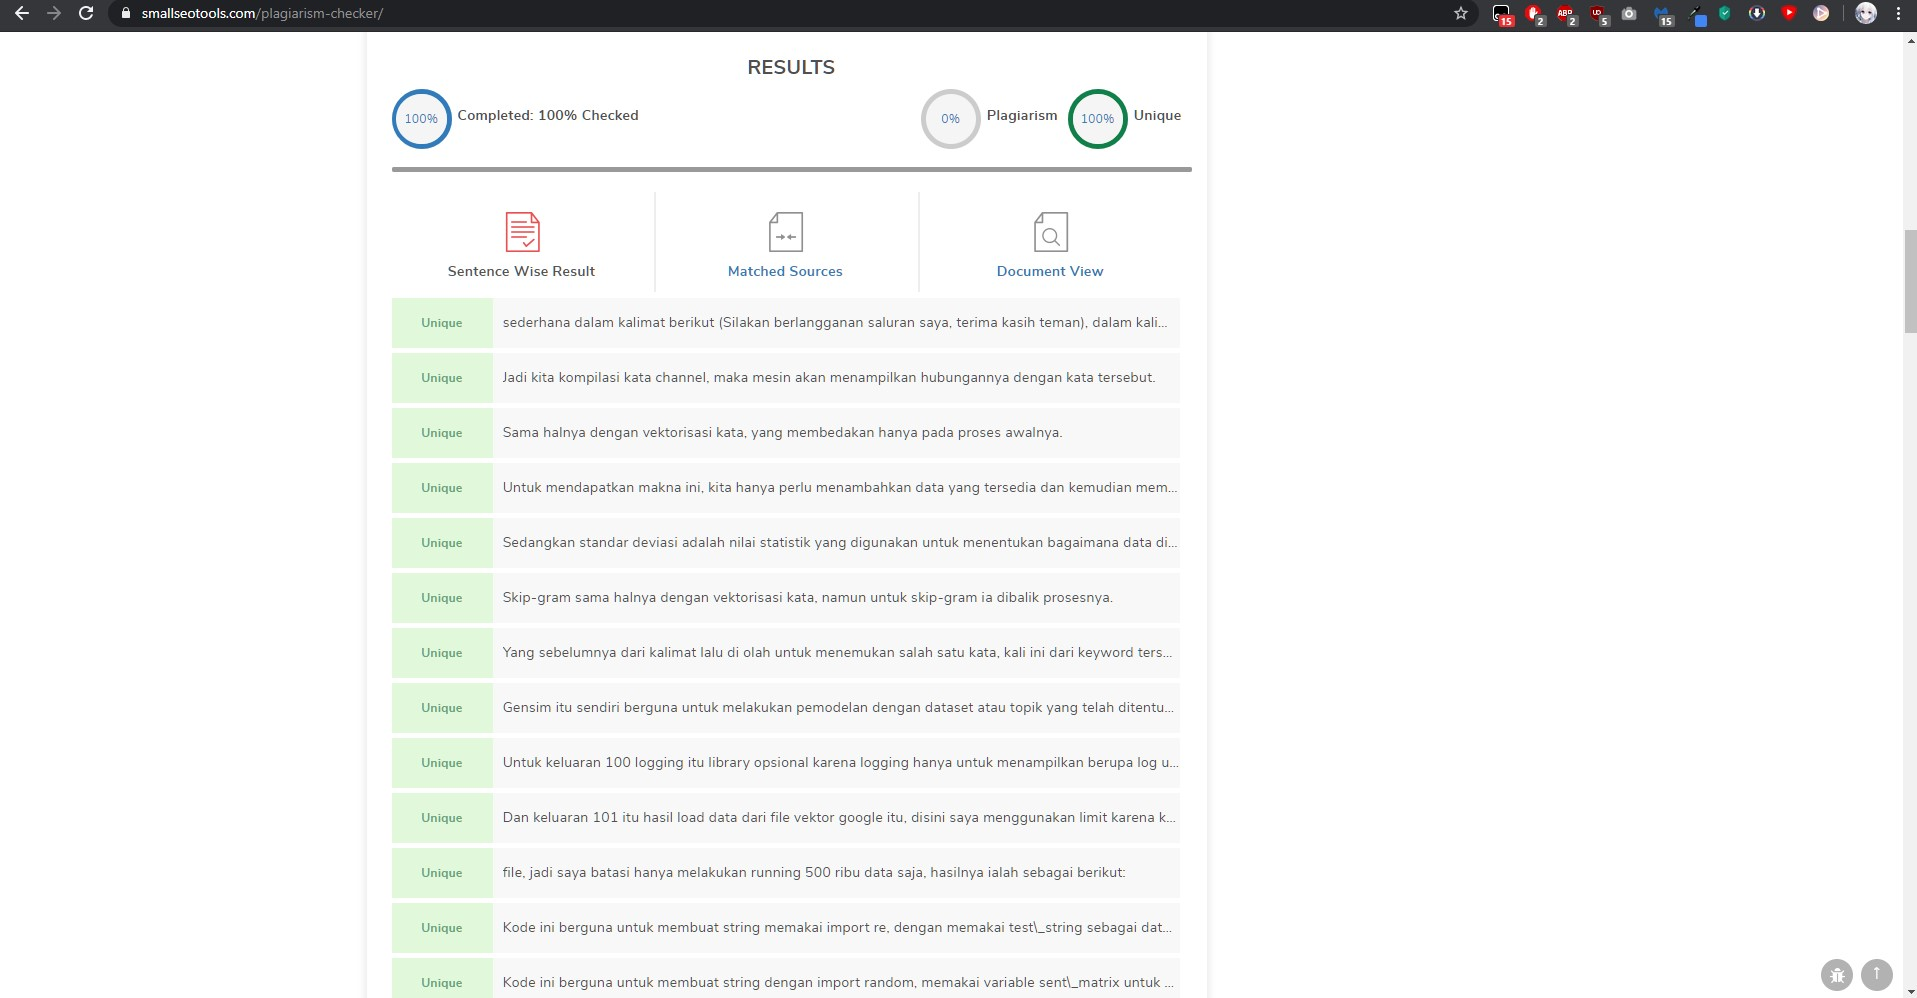
\includegraphics[width=4cm]{figures/1174066/5/plagiat.jpg}
	\centering
	\caption{Bukti Tidak Plagiat}
\end{figure}

\subsection{Link Youtube}
https://youtu.be/AtLNMwxCUSk